% Une ligne commentaire débute par le caractère « % »

\documentclass[a4paper]{article}

% Options possibles : 10pt, 11pt, 12pt (taille de la fonte)
%                     oneside, twoside (recto simple, recto-verso)
%                     draft, final (stade de développement)

\usepackage[utf8]{inputenc}   % LaTeX, comprends les accents !
\usepackage[T1]{fontenc}      % Police contenant les caractères français
\usepackage[francais]{babel}
\usepackage{fullpage}
\usepackage{multicol}
\usepackage{hyperref}
\hypersetup{
    colorlinks=true,
    linkcolor=blue,
    filecolor=magenta,      
    urlcolor=red
    }
\usepackage{bookmark}
\usepackage{blindtext}
\setlength\columnsep{30pt}



\usepackage{graphicx}  % pour inclure des images
\graphicspath{ {rapport/img/} }

%\pagestyle{headings}        % Pour mettre des entêtes avec les titres
                              % des sections en haut de page

\title{  Projet : Inteco\\Programmation mobile}
\author{Mohamad Satea Almallouhi - Tony Nguyen\\\emph{M1 Génie Logiciel}\\Faculté des Sciences\\Université de Montpellier.}
\date{12 mai 2024}



\begin{document}
    \maketitle
    \begin{center}
        
\includegraphics[height=.95\textwidth]{kobeni}
    \end{center}

    \begin{abstract}     % Résumé du travail
      \emph{Durant cet exercice, nous avons vue l'utilisation des Fragments, ModelView et MutableLiveData.}
    \end{abstract}
    \newpage
    %\dominitoc  % initializer les minitoc
    \tableofcontents
    \section*{Introduction}
            \addcontentsline{toc}{section}{Introduction}
            \paragraph{}
                Dans le cadre de l'Unité d'Enseignement Programmation Mobile, nous allons vous parler de notre avancé par rapport à l'application d'intérim.
            \paragraph{}
                Les fonctionnalités implémentés sont la connection et l'inscription ainsi que la récupération d'un Curriculum Vitae (CV).
        \section*{Démonstration vidéo}
            % \addcontentsline{toc}{section}{Démonstration}
            \paragraph{}
                En ligne sur Youtube, à l'adresse URL \url{https://youtu.be/r30-L7iI1IE} une démonstration vidéo de notre travail.
            \paragraph{}
                En ligne sur github, notre dépôt à l'adresse suivante: \url{https://github.com/tony-nguyen1/Inteco/}
        % \section*{Installation}
        %     \addcontentsline{toc}{section}{Démonstration}
        %     \paragraph{}
        %         Vous trouvez les instructions dans le README.md

    \newpage
    \begin{multicols}{2}
        % [
            % To Do
            % \begin{itemize}
            %     \item sc de la bd
            %     \item sc du code pour se connecter 1er page 2e page 3e page, verification de l'email
            %     \item authentification
            %     \item dl et enregistrer un pdf
            %     \item barre de navigation
            % %     \item diagram use case DONE
            % %     \item diagram sequence for synchronisation DONE ~~~
            % %     \item diagram state machine w/ tikz library to describe save function NO
            % %     \item add code picture DONE
            % %     \item add smartphone picture DONE
            % %     \item !!! make an .apk file for easy install, no compilation !!! NO NEED, ALREADY DONE
            % %     \item diagram class observer DONE
            % %     \item diagram class observer specific (Fragment Manager) KO
            %     \item → !!! → vidéo ← !!! ← 
            % \end{itemize}
        %     Faire une vidéo, le rapport avec des screenshot des résultats et du code et enfin un read.md(instruction). En plus, pour le bonus, faire une belle application, des tests unitaires, utiliser Kotlin, faire le rapport en Latex.
        % ]
        \section{Backend avec Firebase}
        \subsection{Sign up - Job Seeker}
        \paragraph{}
        Afin de créer un compte, vous devez entrer vos informations petit à petit sur 3 pages successives. 
        
        La 1er page demande une adresse mail et un mot de passe. Nous considérons les adresses mail comme unique. C'est pourquoi si l'adresse est déjà dans la base de données, l'utilisateur ne peut poursuivre son inscription.
        \noindent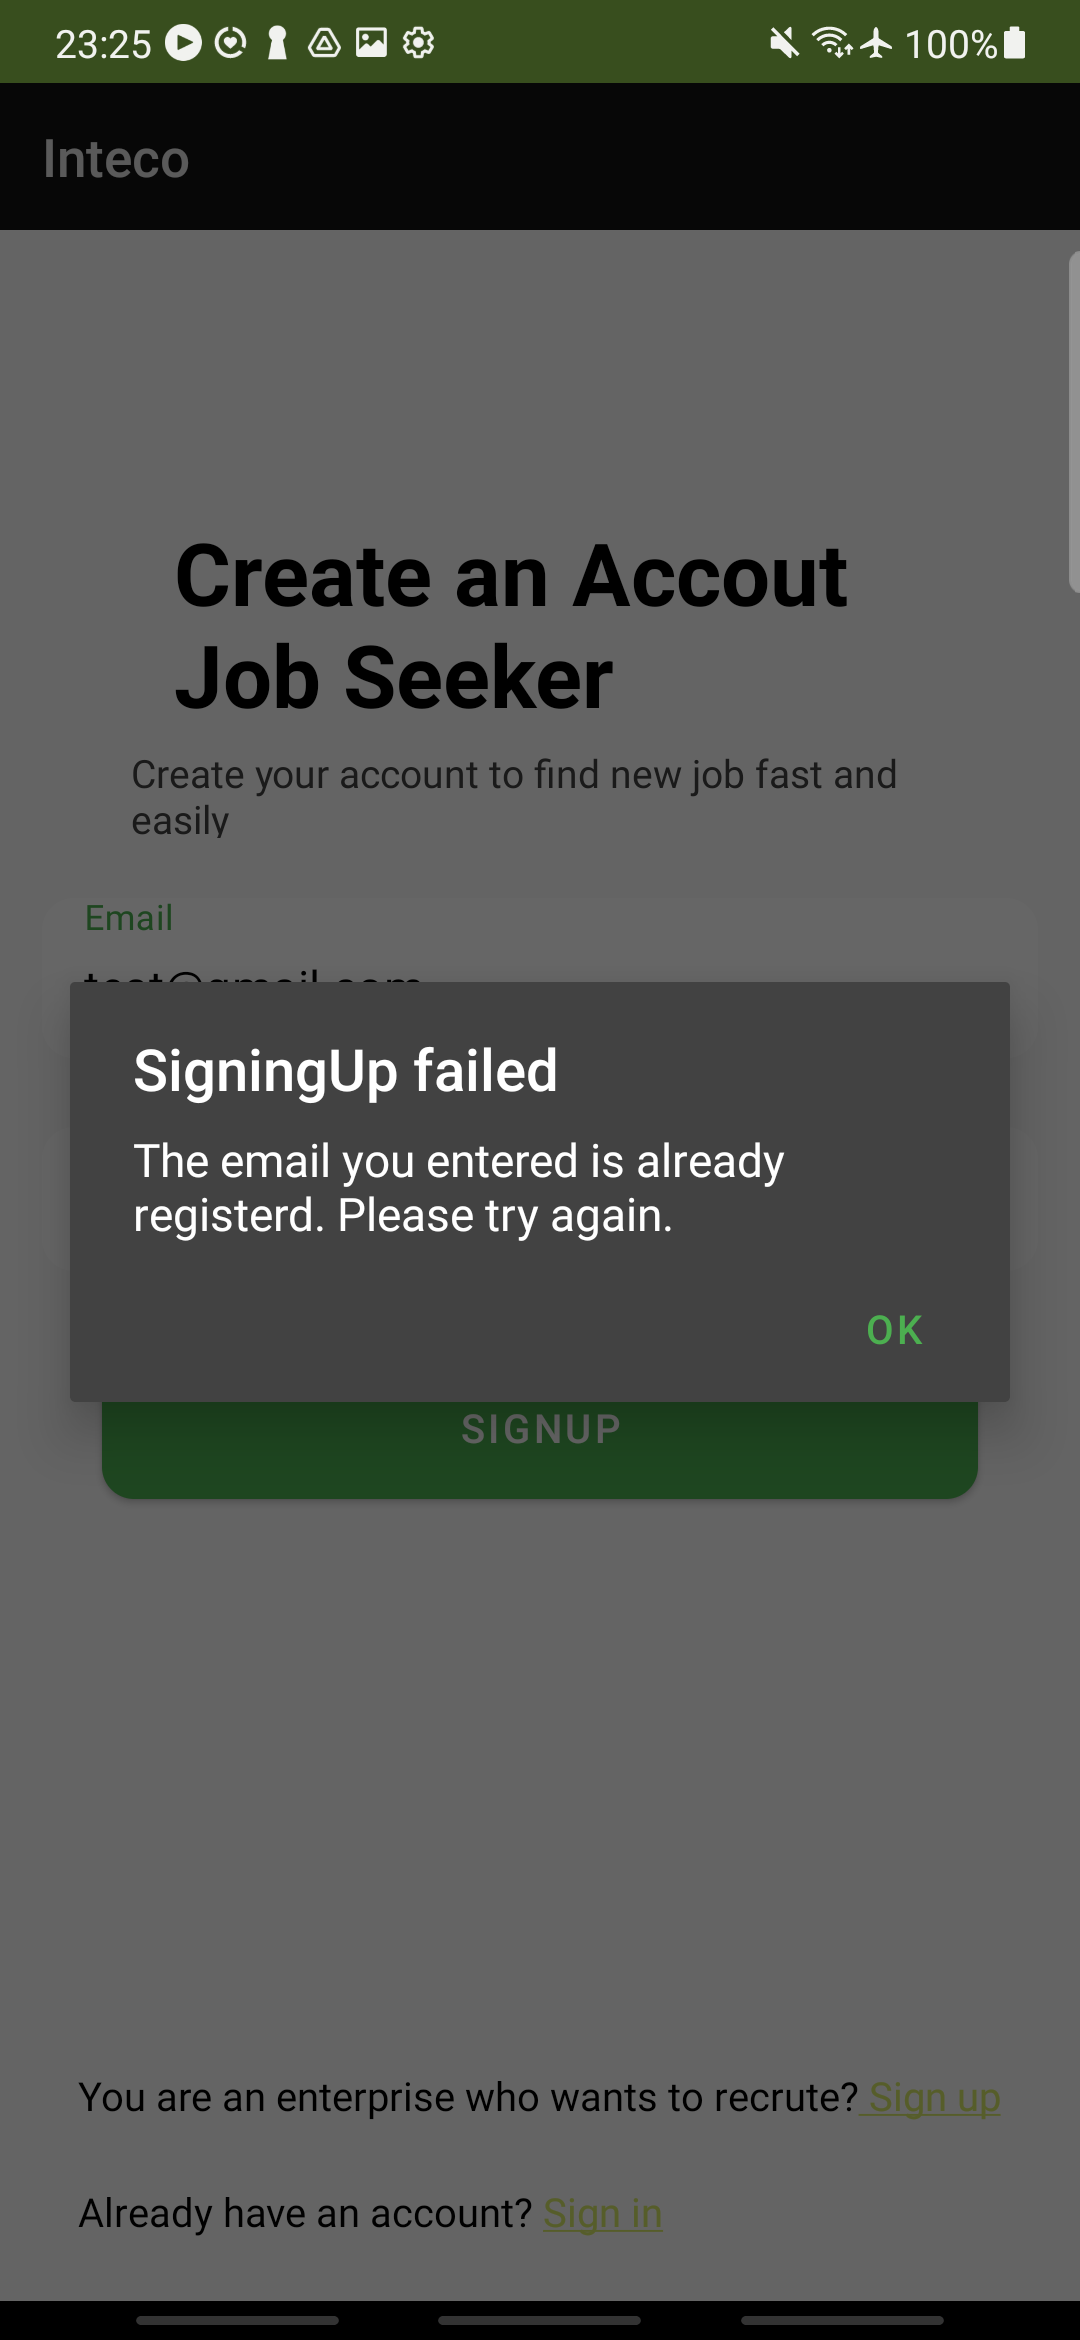
\includegraphics[width=.49\textwidth]{signUpFail}
        \noindent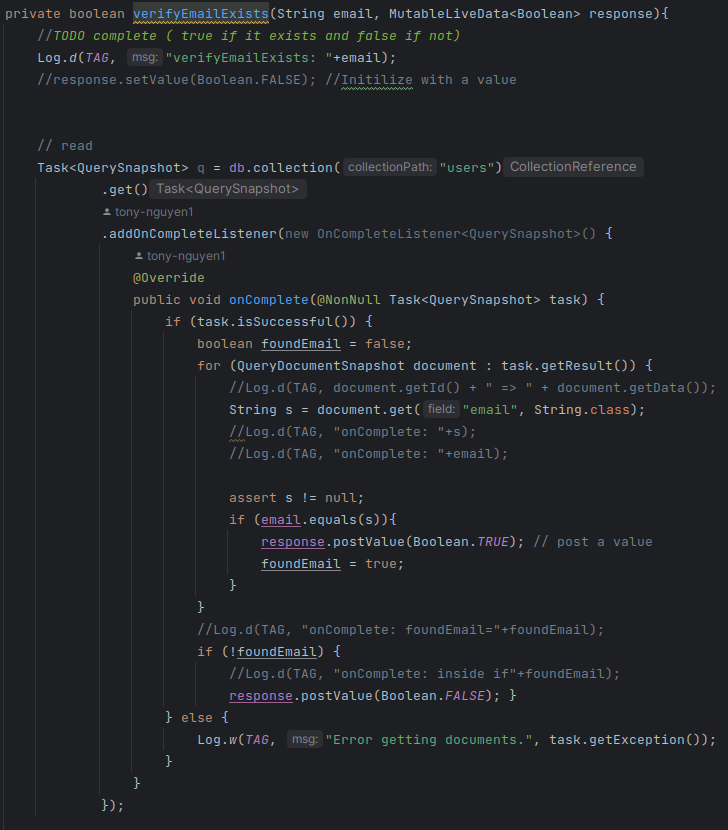
\includegraphics[width=.49\textwidth]{codeVerificationEmail}

        À la dernière page, en appuyant sur le boutton "SIGN UP", le compte est créer. On crée un nouvelle utilisateur avec createUserWithEmailAndPassword(), une fonction qui comunique avec le service Authentification de Firebase. Puis, une fois fait, on enregistre les informations de l'intérimaire dans la BD Firestore. 
        \noindent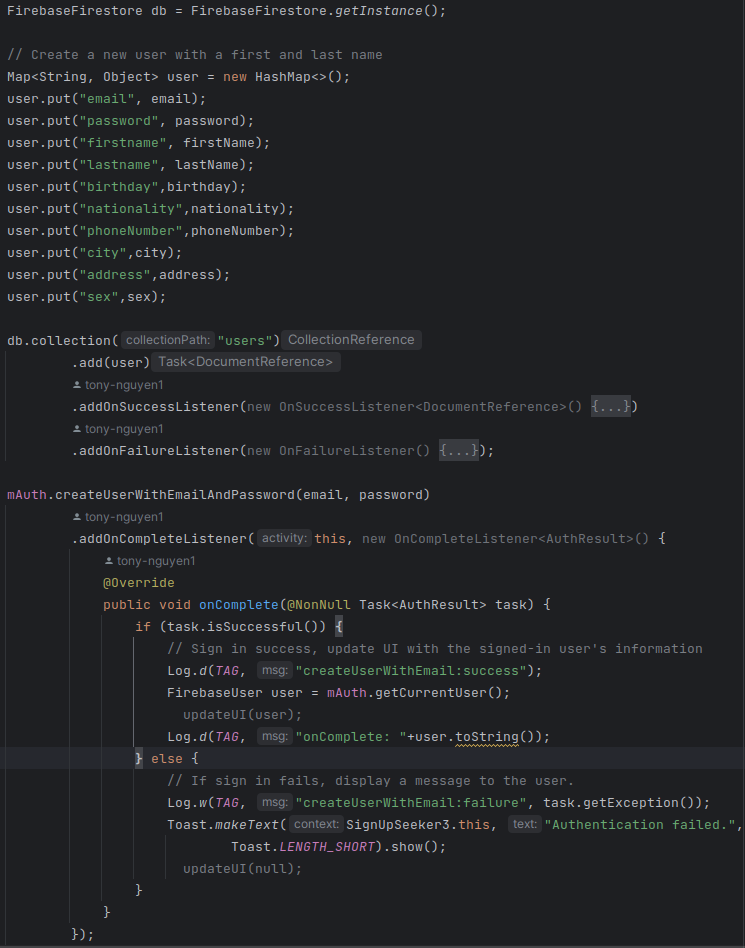
\includegraphics[width=.49\textwidth]{codeSignUp}
        \subsection{Login}
        \paragraph{}
        Pour réaliser la connection, nous avons fait un simple appel au service d'Authentification fournit par Google Firebase. 
        \noindent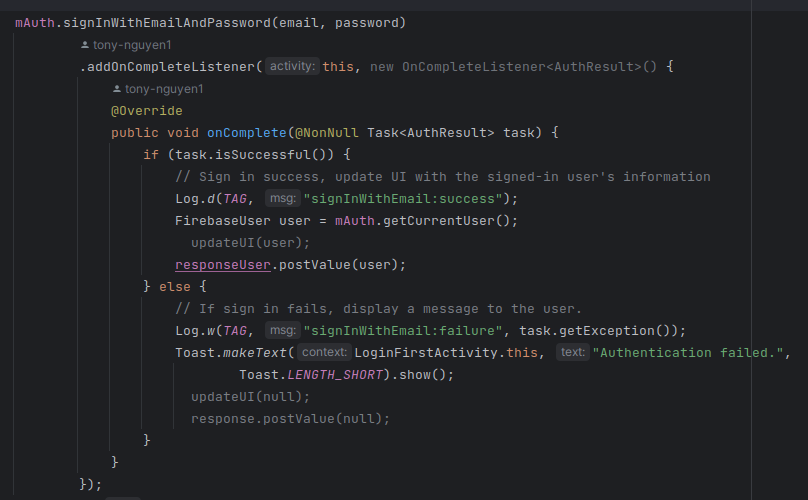
\includegraphics[width=.49\textwidth]{codeSignInA}
        
        Ensuite, nous fesons un appel à la base de données Firestore pour récupérer les informations de ce compte.
        \noindent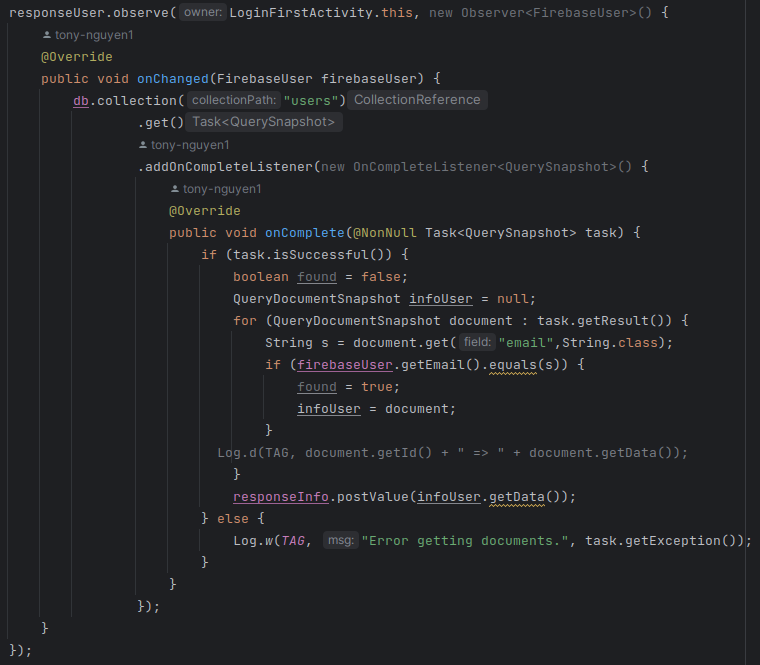
\includegraphics[width=.49\textwidth]{codeSignInB}
        \noindent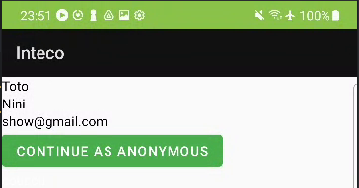
\includegraphics[width=.49\textwidth]{connected}
        \subsection{Récupération d'un document}
        \paragraph{}
        En ce qui concerne la récupération de document comme les CV et lettre de motivation, nous utilisons Firebase Storage. Il nous suffit de faire un appel à la fonction getFile() pour télécharger notre document.
        \noindent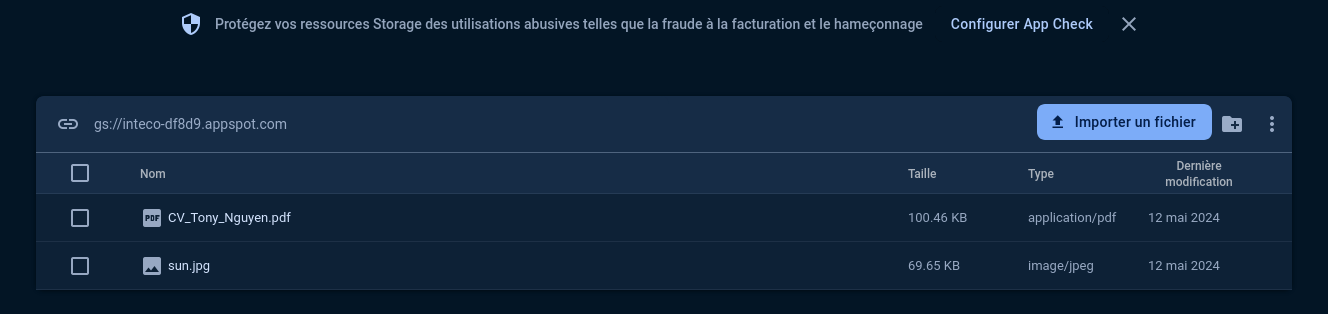
\includegraphics[width=.49\textwidth]{screenshotConsoleFirebaseStorage}
        \noindent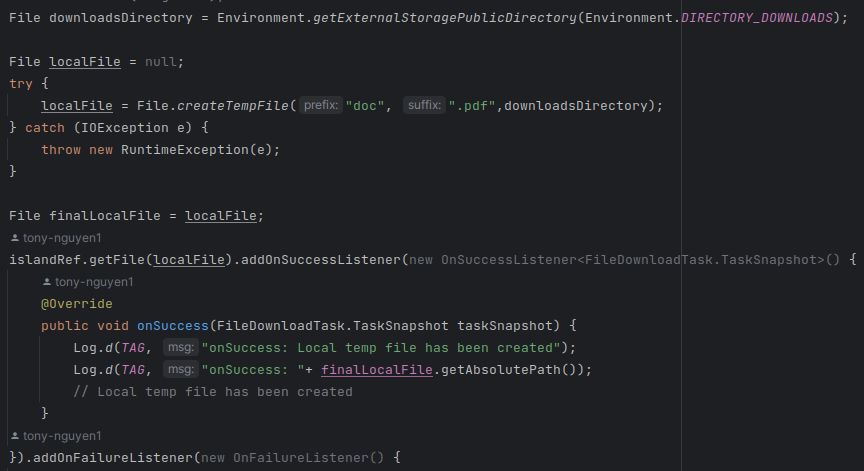
\includegraphics[width=.49\textwidth]{codeDownload}
        \noindent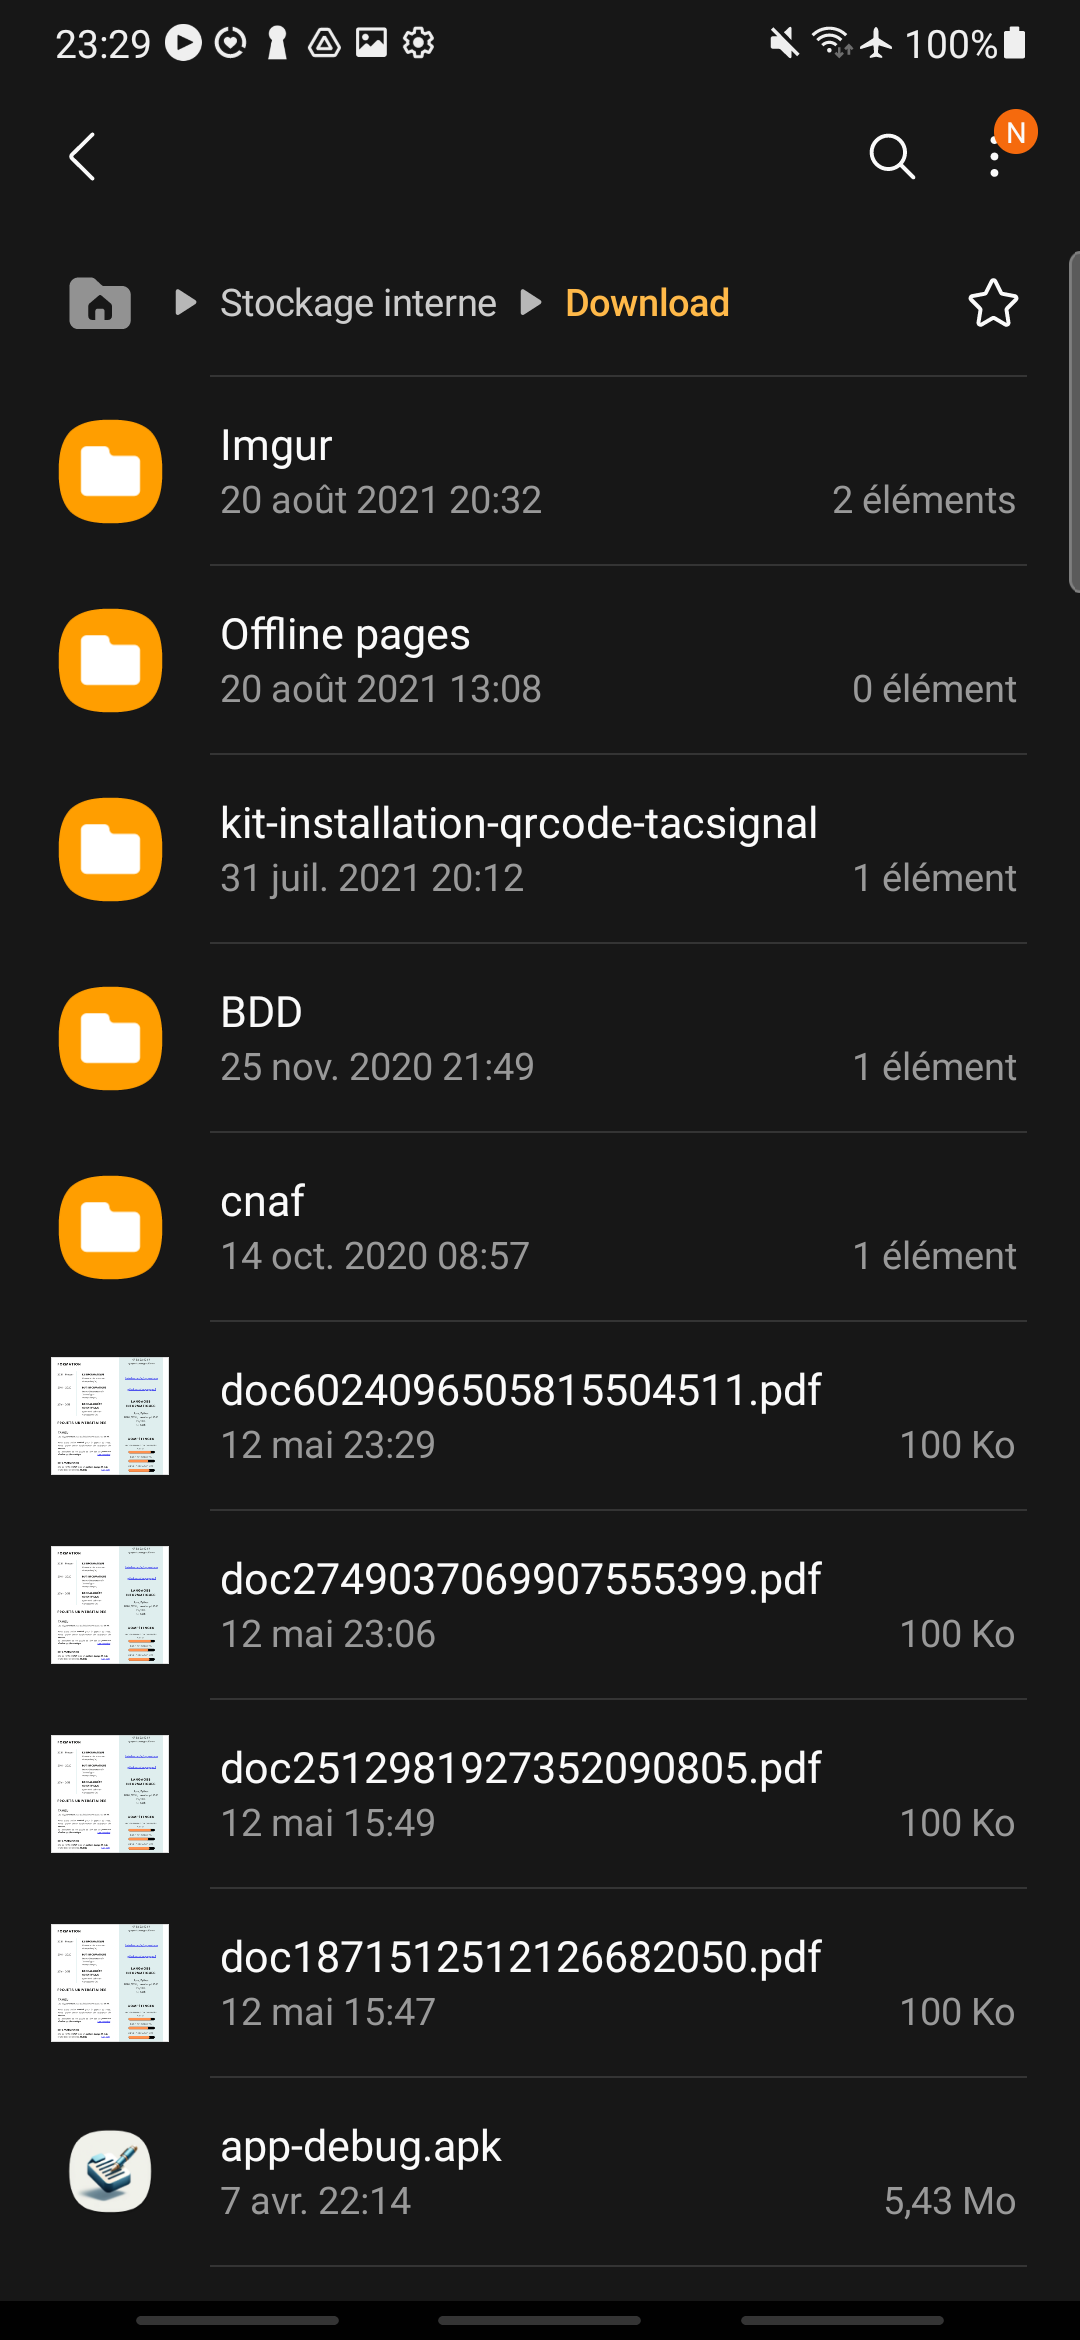
\includegraphics[width=.49\textwidth]{downloadDir}
        \section{Barre de navigation}
        Pour réaliser, la barre de navigation, nous avons utilisé des balises déjà existantes.
        \noindent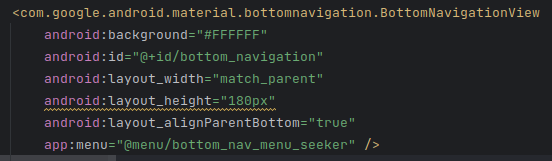
\includegraphics[width=.49\textwidth]{xmlNavBarA}
        \noindent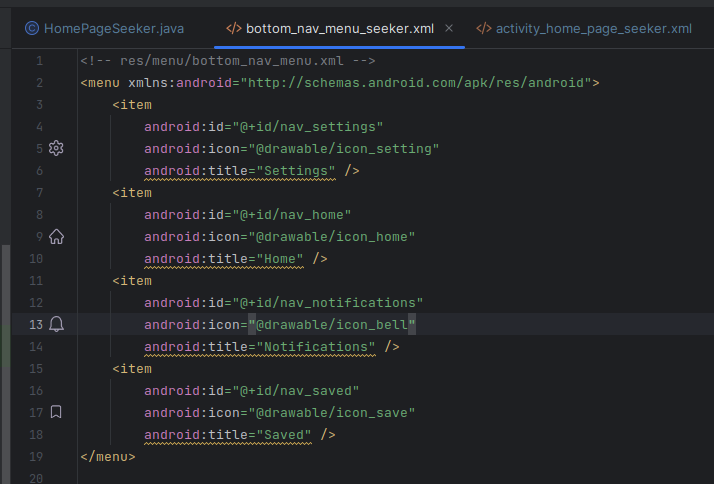
\includegraphics[width=.49\textwidth]{xmlNavBarB}
        \noindent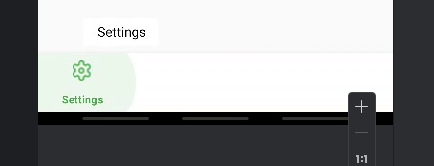
\includegraphics[width=.49\textwidth]{navBar}
        \section{Barre de navigation}
        \paragraph{Settings}
        Le fragment Settings affiche présentes les différentes valeurs de l'entreprise. Ainsi que la fonctionnalités de modification de ces valeurs.


        %     \subsection{Communication entre fragment}
                
        %     \subsection{La synchronisation et mise à jour}
        %     \subsection{Observer}
        % \section{Persistance}
        %     \subsection{(Re-)Saisie automatique}
        % \section{Réseau}
        %     Cet exerice n'a pas été réalisé.
        % \section{Service}
        \section{Conclusion}
    \end{multicols}
\end{document}